\XeTeXinputencoding cp1250
% ********** Appendix 1 **********
\chapter{Diagrame UML}
\label{sec:appendix1}
�n aceast� anex� apar diagramele UML detaliate ale proiectului cytrus. Organizarea este �n func�ie de namespace-urile claselor, dup� cum urmeaz�:
\begin{figure}[htbp]
\numberwithin{figure}{chapter}
\centering
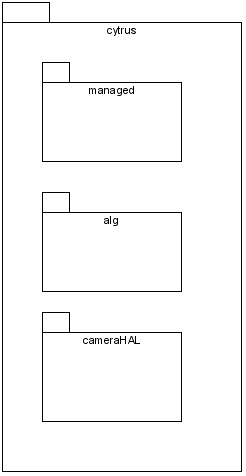
\includegraphics[scale=0.5]{app1/cytrus.png}
\caption{cytrus}
\label{fig:app1:cytrus}
\end{figure}
\begin{figure}[htbp]
\numberwithin{figure}{chapter}
\centering
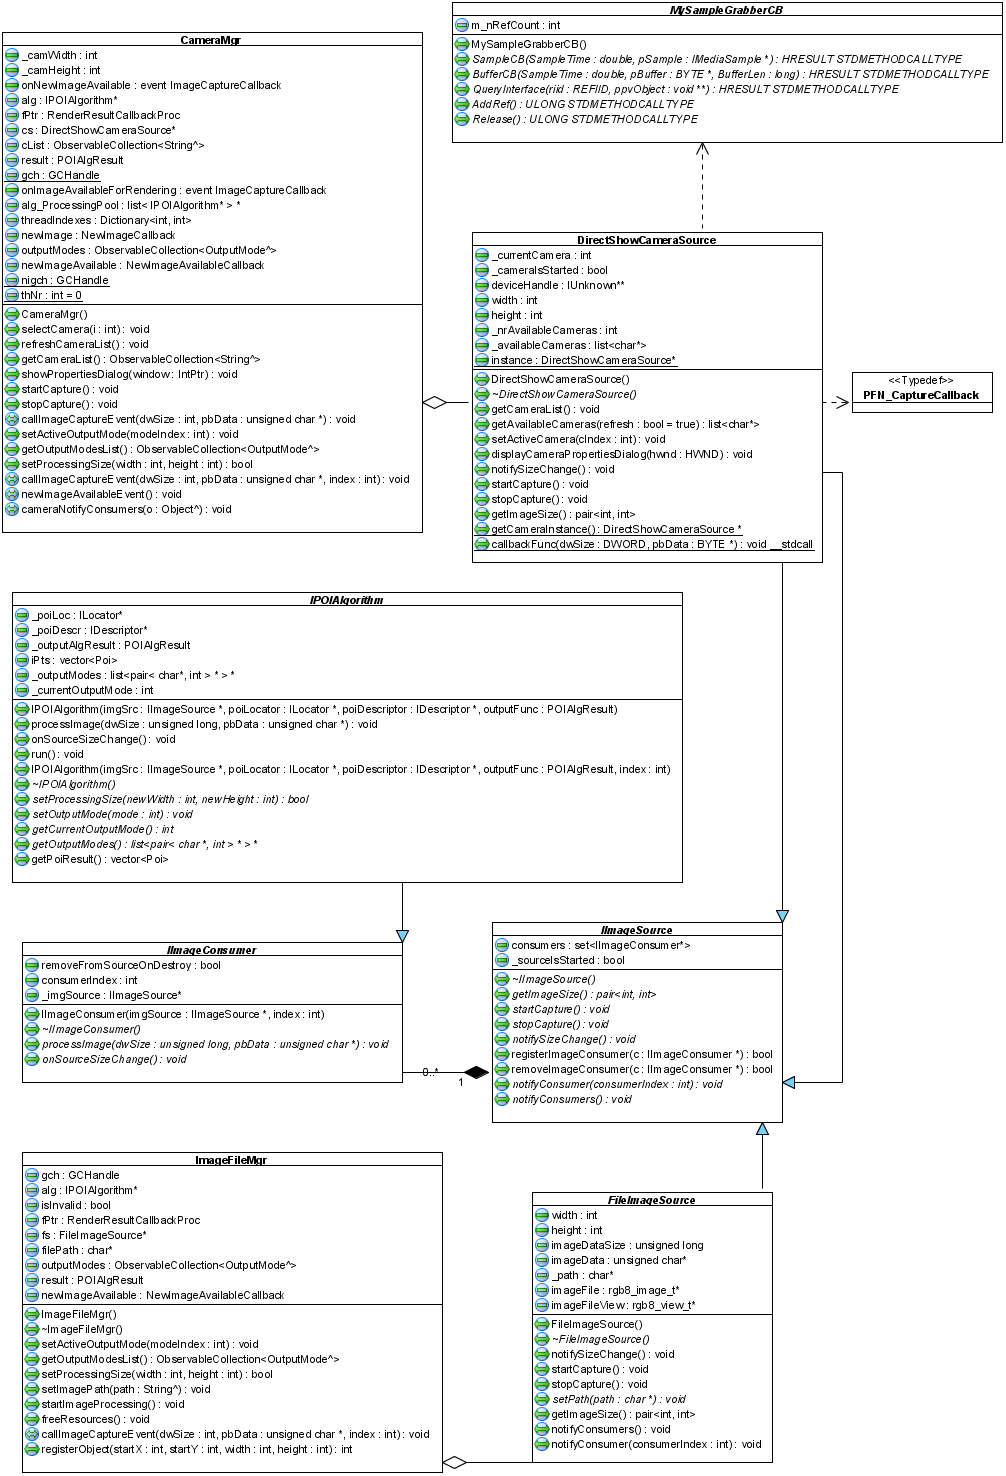
\includegraphics[scale=0.45]{app1/cytrus.cameraHAL.png}
\caption{cytrus::cameraHAL}
\label{fig:app1:cameraHAL}
\end{figure}
\begin{landscape} 
\begin{figure}[htbp]
\numberwithin{figure}{chapter}
\centering
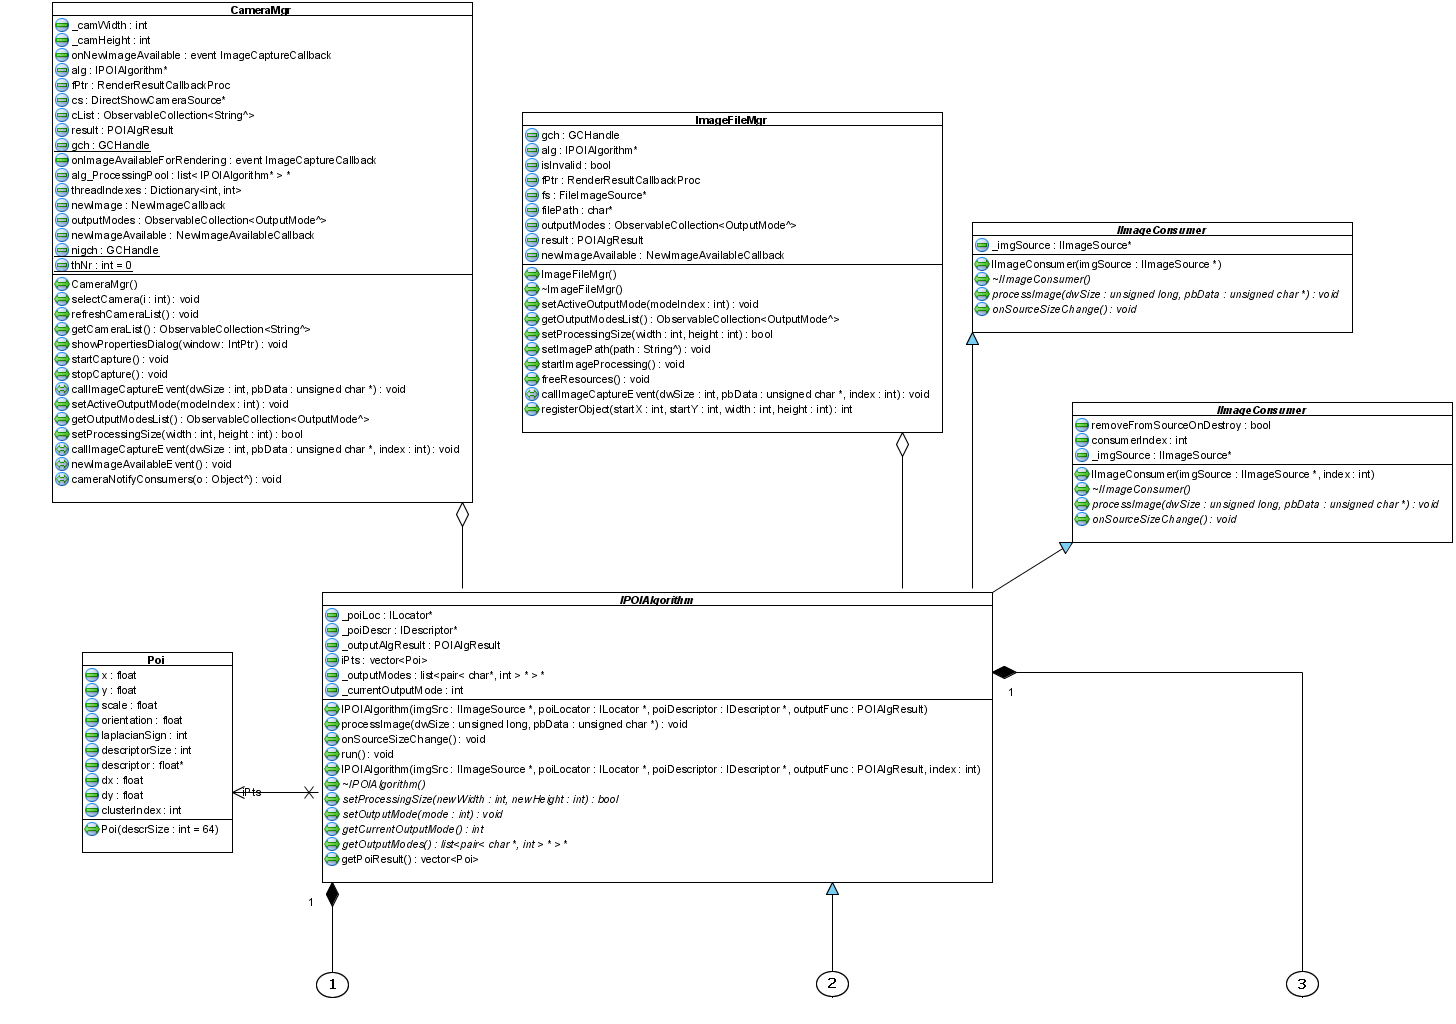
\includegraphics[scale=0.45]{app1/cytrus.alg1.png}
\end{figure}
\end{landscape}
\begin{landscape} 
\begin{figure}[htbp]
\numberwithin{figure}{chapter}
\centering
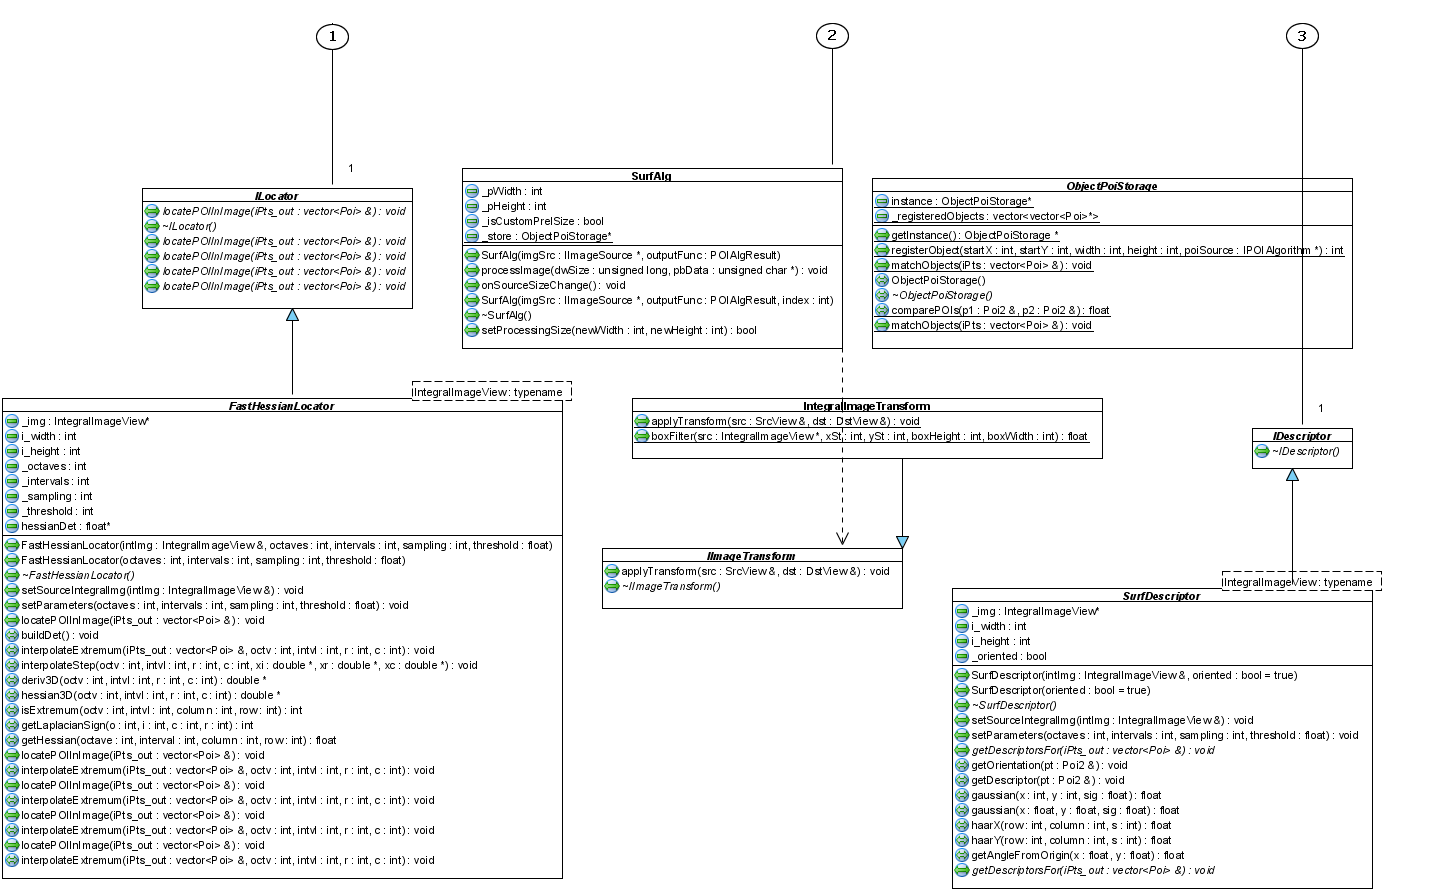
\includegraphics[scale=0.45]{app1/cytrus.alg2.png}
\caption{cytrus::alg}
\label{fig:app1:alg}
\end{figure}
\end{landscape}
\begin{figure}[htbp]
\numberwithin{figure}{chapter}
\centering
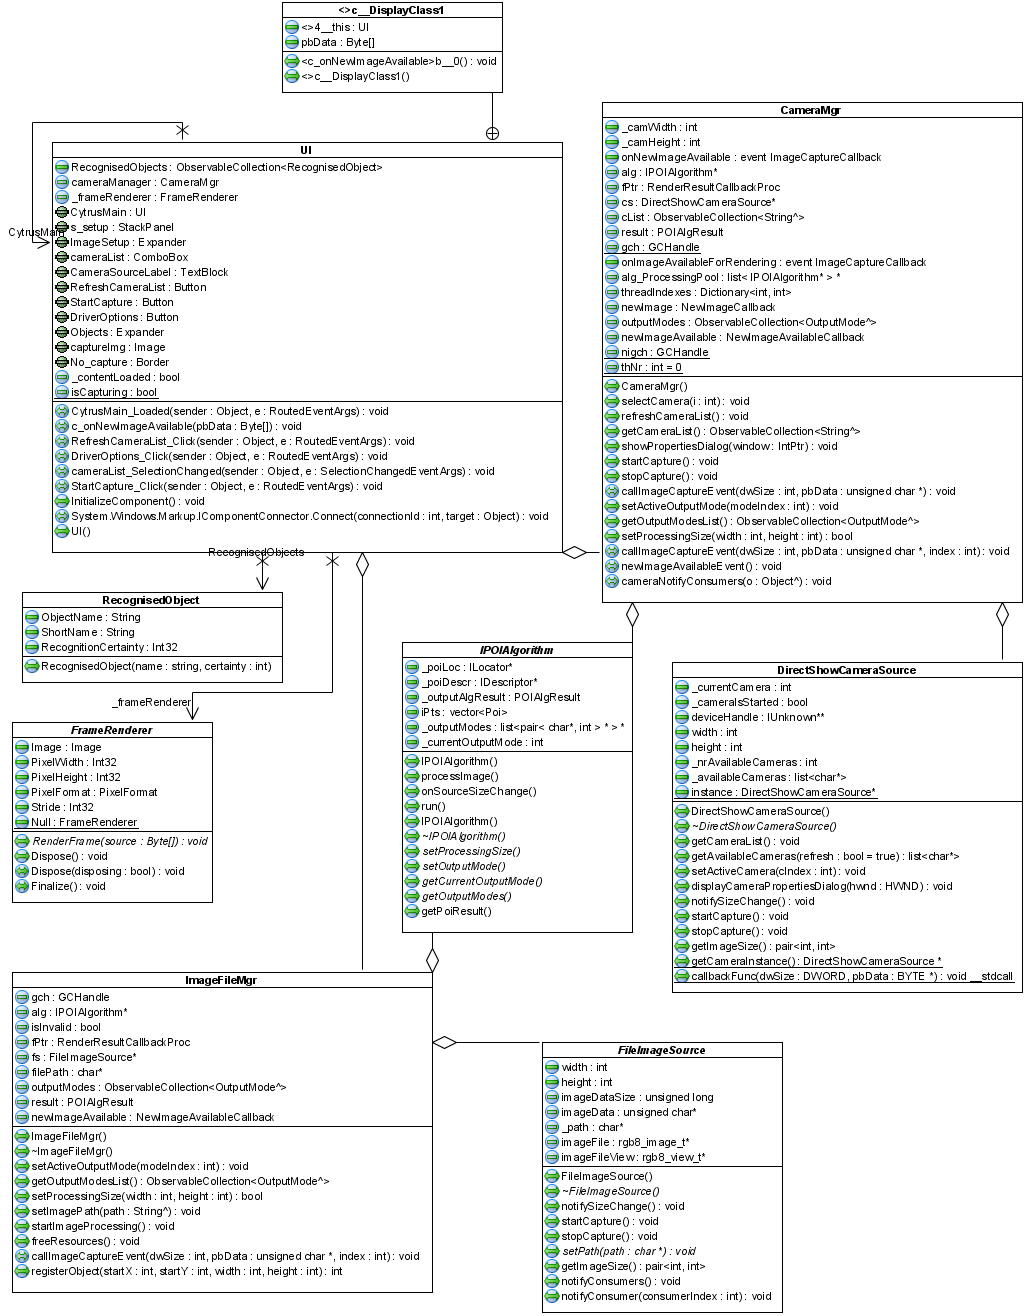
\includegraphics[scale=0.45]{app1/cytrus.managed.png}
\caption{cytrus::managed}
\label{fig:app1:managed}
\end{figure}
\begin{figure}[htbp]
\numberwithin{figure}{chapter}
\centering
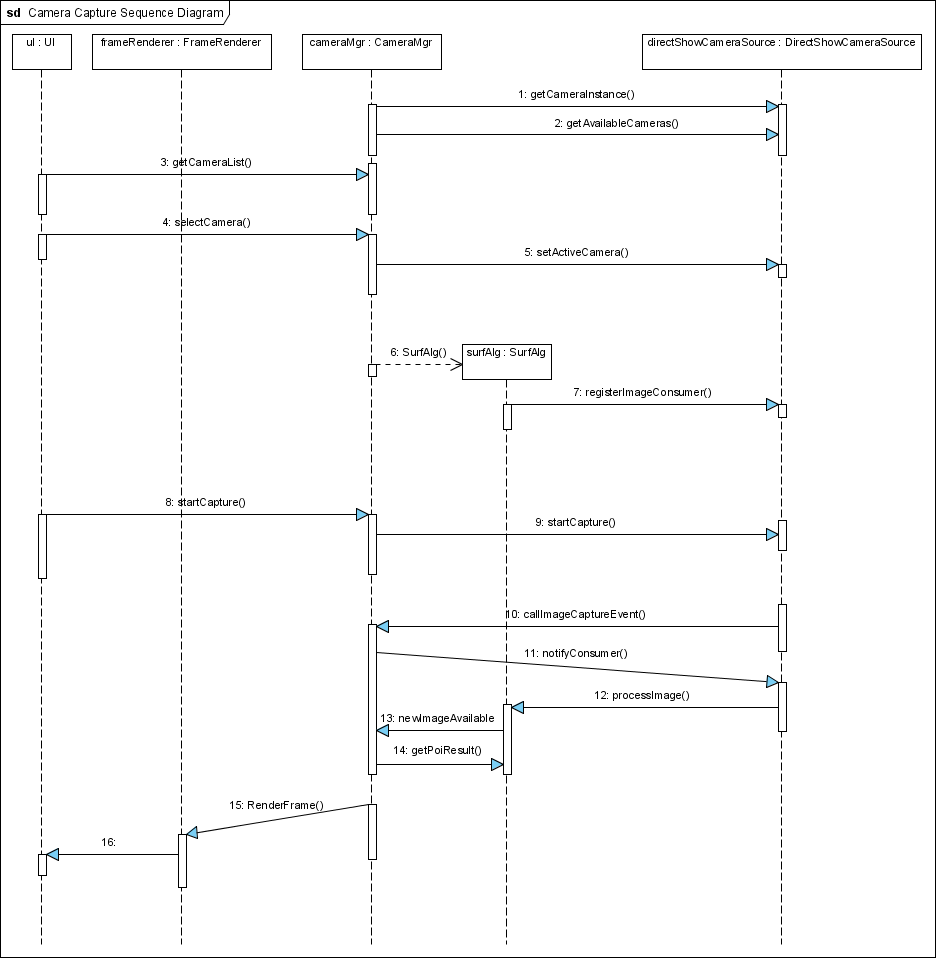
\includegraphics[scale=0.45]{app1/cameraSeq.png}
\caption{Diagram� de secven�� pentru procedura de achizi�ie a imaginilor (simplificat)}
\label{fig:app1:seq}
\end{figure}
% ********** End of appendix **********
